
Within the CASTRO distribution, there is the capability to ``grow'' a checkpoint file so 
that a calculation can be restarted in a larger domain covered by grid cells a factor of
two or four coarser than the existing coarsest level.  Instructions for how to
do so are in the Parallel/Castro/ConvertCheckpoint/README file and are included here.
Upon restart the existing data in the checkpoint file will be used to fill the region of the previous 
computational domain, and the new regions will be filled by some other means, typically
interpolation from a 1D model file.

\section{Star in Corner ({\bf star\_at\_center = 0}) }

In this section we consider the case where the star (or feature of interest) 
is centered at the lower left corner of the domain, e.g. you are modeling only one 
quarter of the star in 2D, or an octant of the star in 3D.  Then you only want
to grow the domain in the ``high side'' directions (e.g., to the upper right).

\subsection{Converting the Checkpoint File}

Let's say you have a checkpoint file, {\em chk00100},  say, with 5 levels of refinement 
and a (real) problem domain size $P$ and (integer) domain size $D$ at level 0.  

The inputs file that created this might have contained:

\begin{itemize}

\item {\bf max\_step}      = 100

\item {\bf amr.max\_level} = 5

\item {\bf amr.n\_cell}    = D D

\item {\bf geometry.prob\_lo} = 0 0

\item {\bf geometry.prob\_hi} = P P

\item {\bf amr.ref\_ratio}    = 4 4 4 4

\end{itemize}

Now let's suppose that you want to grow the domain by a factor of 8 and cover that
new larger domain with a level that is a factor of 2 coarser than the existing level 0 grids.

\begin{enumerate}

\item First, set DIM = in the GNUmakefile, and type  "make" in the ConvertCheckpoint directory.
This will make an executable from the Embiggen.cpp code.

\item Run the embiggening code as follows:

Embiggen2d.Linux.Intel.Intel.ex {\bf checkin}=chk00100 {\bf checkout}=newchk00050
{\bf ref\_ratio}=2 {\bf grown\_factor}=8 {\bf star\_at\_center}=0

(Your executable may have a slightly different name depending on the compilers you
built it with.)

This will create a new checkpoint directory, called {\it newchk00050}, that represents a simulation
with {\it one} additional level of refinement {\it coarser} than the previous level 0 grids by
a factor of {\bf ref\_ratio} (in this case, 2).   
The new domain will be a factor of {\bf grown\_factor} (in this case, 8) larger than the previous domain.

Note that {\bf ref\_ratio} must be 2 or 4, because those are the only acceptable values of {\bf ref\_ratio}
in CASTRO.

{\bf grown\_factor} can be any reasonable integer; I've only tested 2, 3, 4 and 8.  It does not need
to be a multiple of 2.

\end{enumerate}

\subsection{Restarting from a Grown Checkpoint File}

You should now be able to restart your calculation using {\em newchk00050}.

Your inputs file should now contain lines like:

\begin{itemize}

\item {\bf max\_step}      = 51

\item {\bf amr.restart} = newchk00050

\item {\bf amr.max\_level} = 6

\item {\bf amr.n\_cell}    = 4D 4D

\item {\bf geometry.prob\_lo} =  0  0

\item {\bf geometry.prob\_hi} = 8P 8P

\item {\bf castro.grown\_factor} = 8

\item {\bf castro.star\_at\_center} = 0

\item {\bf amr.ref\_ratio}    = 2 4 4 4 4

\end{itemize}

IMPORTANT:

\begin{enumerate}

\item Unlike earlier, you may now set {\bf amr.max\_level} to be at most one greater than before,
but you need not set it that high.  For example, you could set {\bf amr.max\_level} the same as before
and you would lose data at the finest refinement level.   You may not set {\bf amr.max\_level} = 0,
however, because we have no data at the new level 0 until we average down from the new level 1 after
the restart.

\item You must set {\bf amr.n\_cell} = ({\bf grown\_factor} / {\bf ref\_ratio}) times the previous 
value of {\bf amr.n\_cell}.  In this case {\bf amr.n\_cell} = (8/2)*D = 4D.

\item You must set {\bf amr.prob\_hi} to be a factor of {\bf grown\_factor} greater than the previous 
value of {\bf amr.prob\_hi}.

\item You must insert the value of {\bf ref\_ratio} used in the Embiggen call as the first
value in the list of {\bf amr.ref\_ratio}, since that will now be the refinement ratio between 
the new level 0 and the new level 1.

\item You must set {\bf castro.grown\_factor} in your inputs file equal to the value of 
{\bf grown\_factor} you used when you called Embiggen*ex so that the CASTRO code knows 
how big the original domain was.

\item Note that if you have run 100 steps at the original level 0, that would be equivalent
to 50 steps at the new level 0 because you coarsened by a factor of 2.  
Thus once you re-start from the new checkpoint directory,
the next step will be 51, not 101.  Make sure to keep track of your plotfiles accordingly.

\item Don't forget to adjust max\_denerr\_lev and comparable variables to control
the number of fine levels you now want.   If you want to have 6 levels of refinement
after restart, then make sure max\_denerr\_lev, etc, are set high enough.  If you
only want to have 5 levels of refinement (where the new level 5 would now be
a factor of ref\_ratio coarser than the previous level 5), make sure to adjust
max\_denerr\_lev accordingly as well.

\end{enumerate}
   
\section{Star at Center of Domain ({\bf star\_at\_center = 1}) }

Now let's assume that the star (or feature of interest) is centered at the center of the
domain in 2D or 3D Cartesian coordinates. We will later consider the case of 2D cylindrical (r-z)
coordinates in which the star is centered at the left midpoint.

\subsection{Converting the Checkpoint File}

Suppose that you want to grow the domain by a factor of 2 and cover that
new larger domain with a level that is a factor of 2 coarser than the existing level 0 grids.

After you build the Embiggen executable, you type:

\begin{itemize}

\item Embiggen2d.Linux.Intel.Intel.ex {\bf checkin}=chk00100 {\bf checkout}=newchk00050 {\bf ref\_ratio}=2 \\
{\bf grown\_factor}=2  {\bf star\_at\_center}=1

\end{itemize}

Note that 
\begin{itemize}

\item {\bf ref\_ratio} must still be 2 or 4

\item {\bf grown\_factor} can only be 2 or 3 in this case.

\end{itemize}

\subsection{Restarting from a Grown Checkpoint File}

Your inputs file for restarting would now look like

\begin{itemize}

\item {\bf max\_step}      = 51

\item {\bf amr.restart} = newchk00050

\item {\bf amr.max\_level} = 6

\item {\bf amr.n\_cell}    = D D

\item {\bf geometry.prob\_lo} = -P/2  -P/2

\item {\bf geometry.prob\_hi} = 3P/2  3P/2

\item {\bf castro.grown\_factor} = 2

\item {\bf castro.star\_at\_center} = 1

\item {\bf amr.ref\_ratio}    = 2 4 4 4 4

\end{itemize}

\subsection{Cylindrical Coordinates}

In the case of 2D cylindrical (r-z) coordinates in which the star is centered at the left edge
but vertical midpoint of the domain, the embiggening procedure is the same as above
(with {\bf star\_at\_center = 1}) but the inputs file for restart is slightly different in that
{\bf geometry.prob\_lo} is modified in the z- but not the r-direction.   If we consider the original
inputs file to look like:

\begin{itemize}

\item {\bf max\_step}      = 100

\item {\bf amr.max\_level} = 6

\item {\bf amr.n\_cell}    = D 2D

\item {\bf geometry.prob\_lo} = 0 0

\item {\bf geometry.prob\_hi} = P 2P

\item {\bf amr.ref\_ratio}    = 4 4 4 4

\end{itemize}

then an inputs file for restart would look like:

\begin{itemize}

\item {\bf amr.restart} = newchk00050

\item {\bf amr.max\_level} = 6

\item {\bf amr.n\_cell}    = D 2D

\item {\bf geometry.prob\_lo} = 0   -P

\item {\bf geometry.prob\_hi} = 2P  3P

\item {\bf castro.grown\_factor} = 2

\item {\bf castro.star\_at\_center} = 1

\item {\bf amr.ref\_ratio}    = 2 4 4 4 4

\end{itemize}


%%%%%%%%%%%%%%%%%%%%%%%%%%%%%%%%%
\begin{figure}[h]
\centering
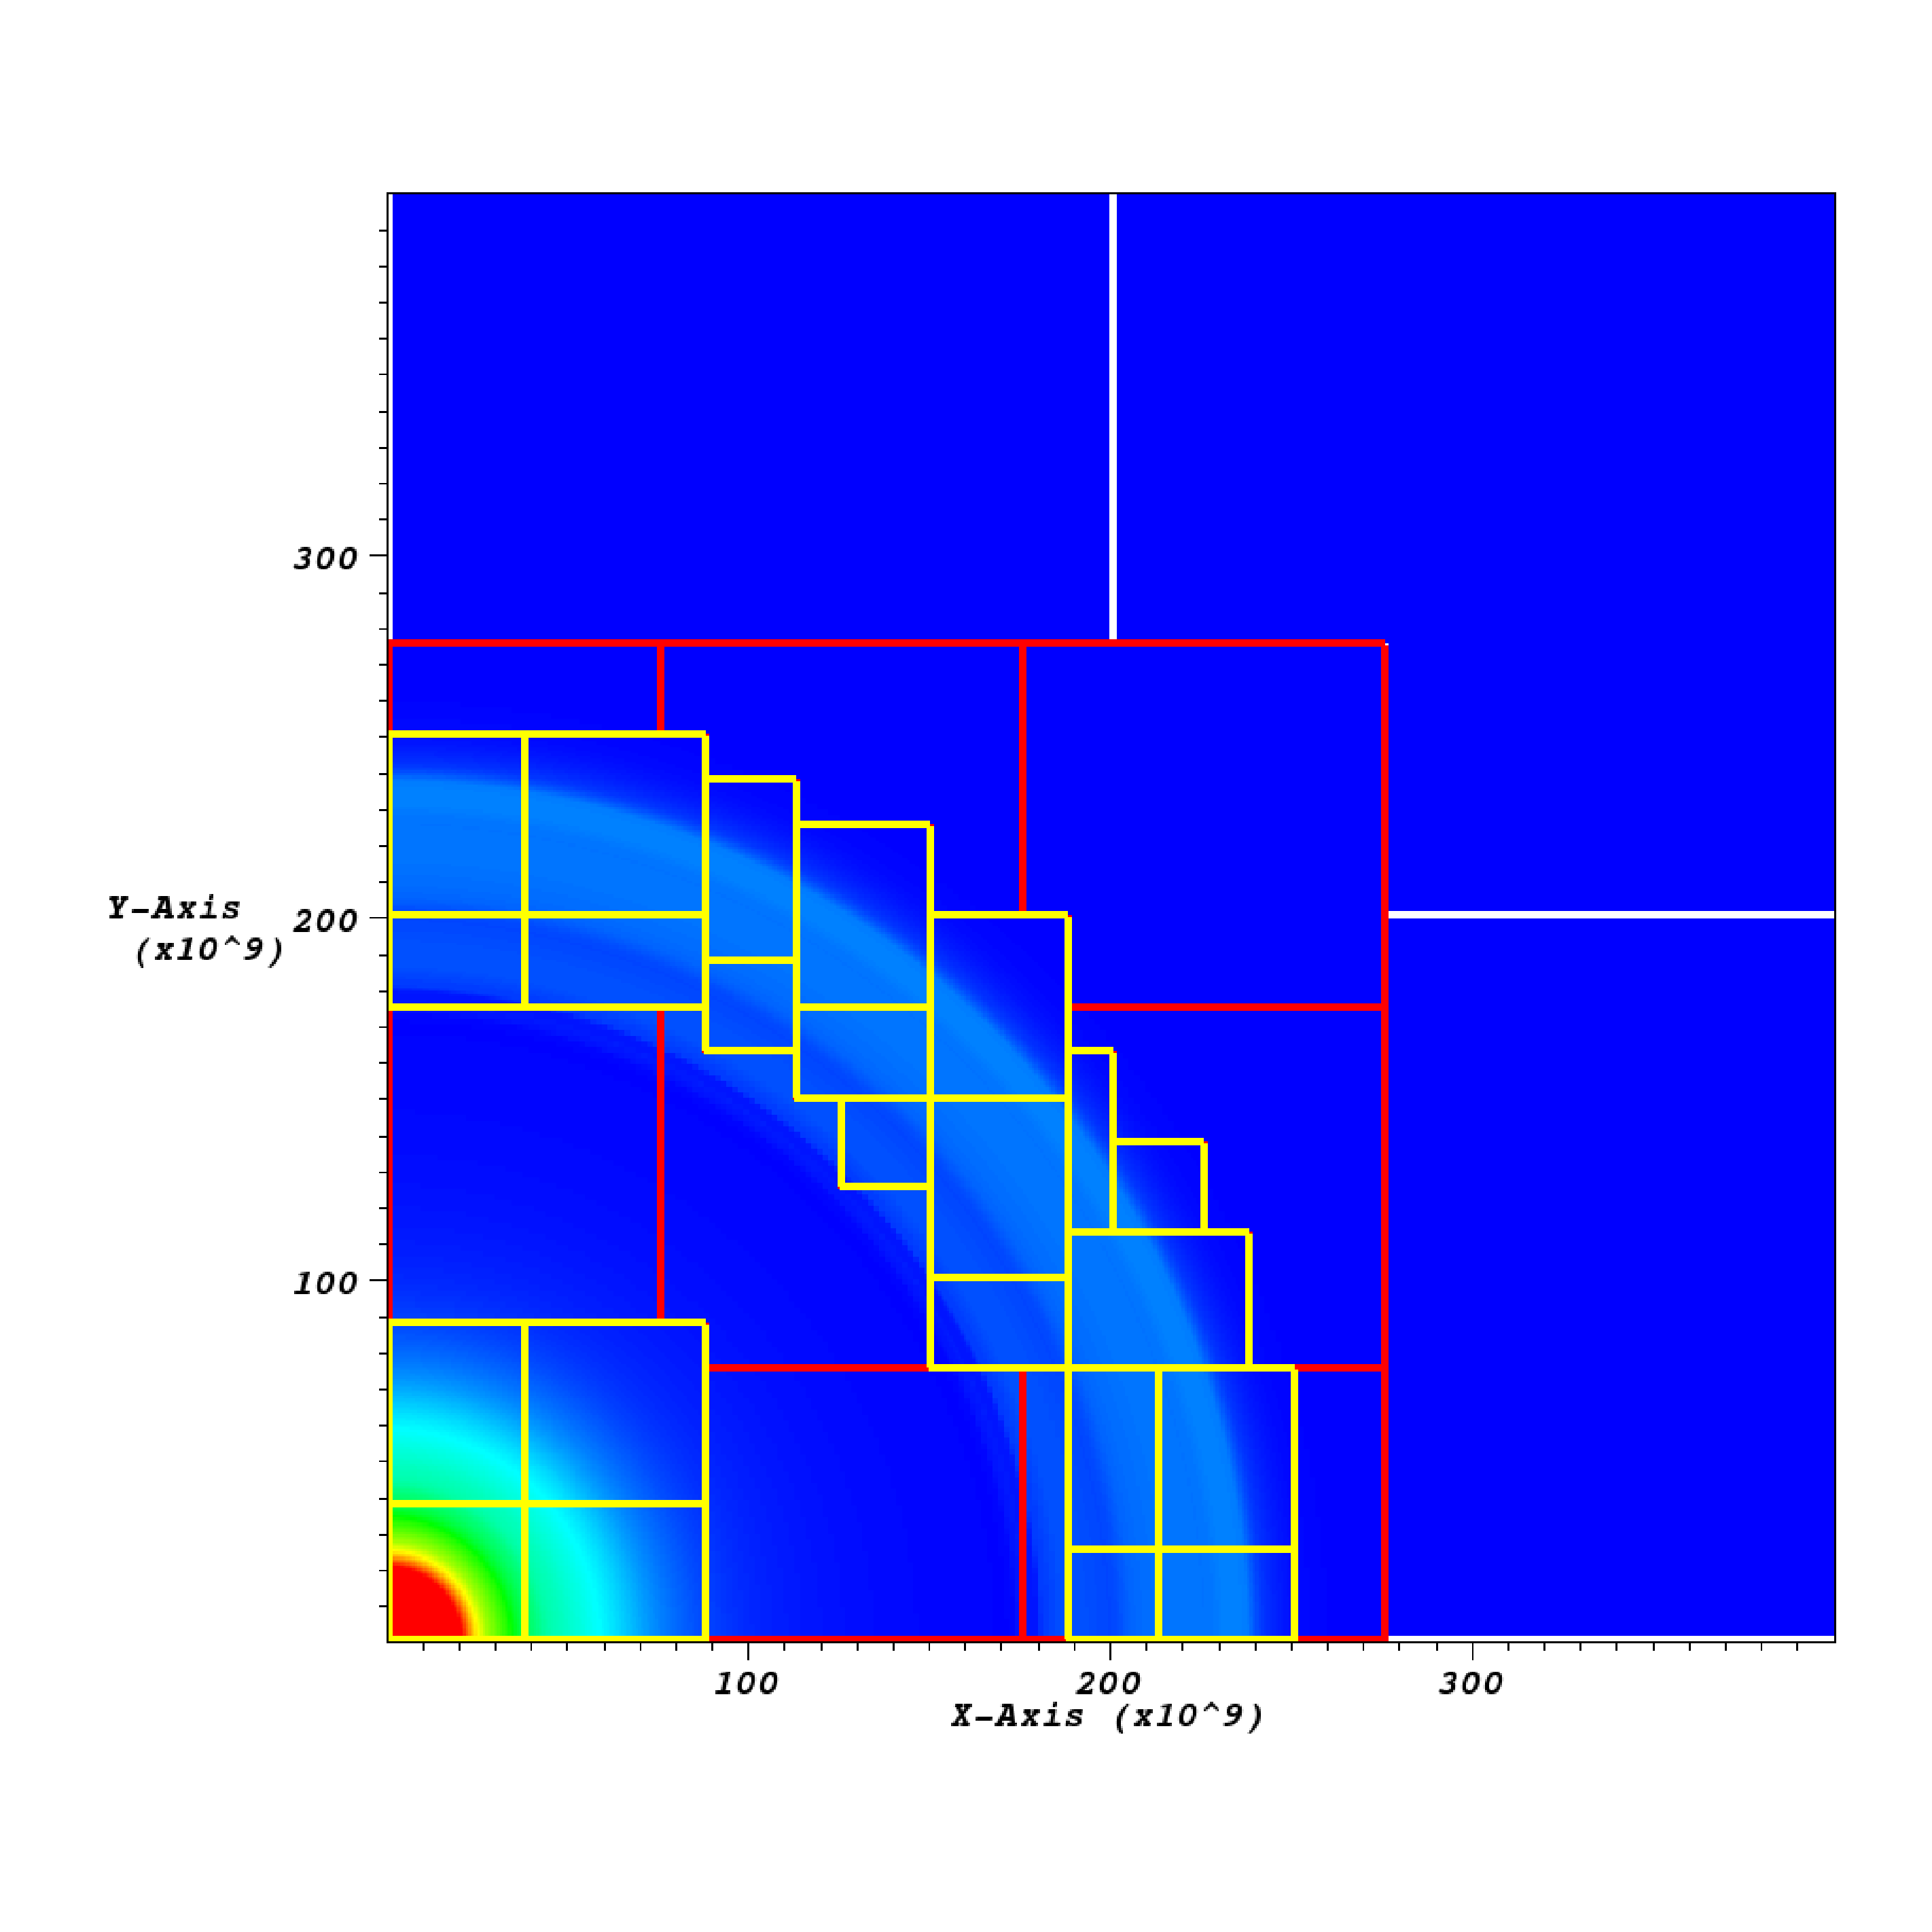
\includegraphics[width=3in]{ConvertCheckpoint/orig_corner}
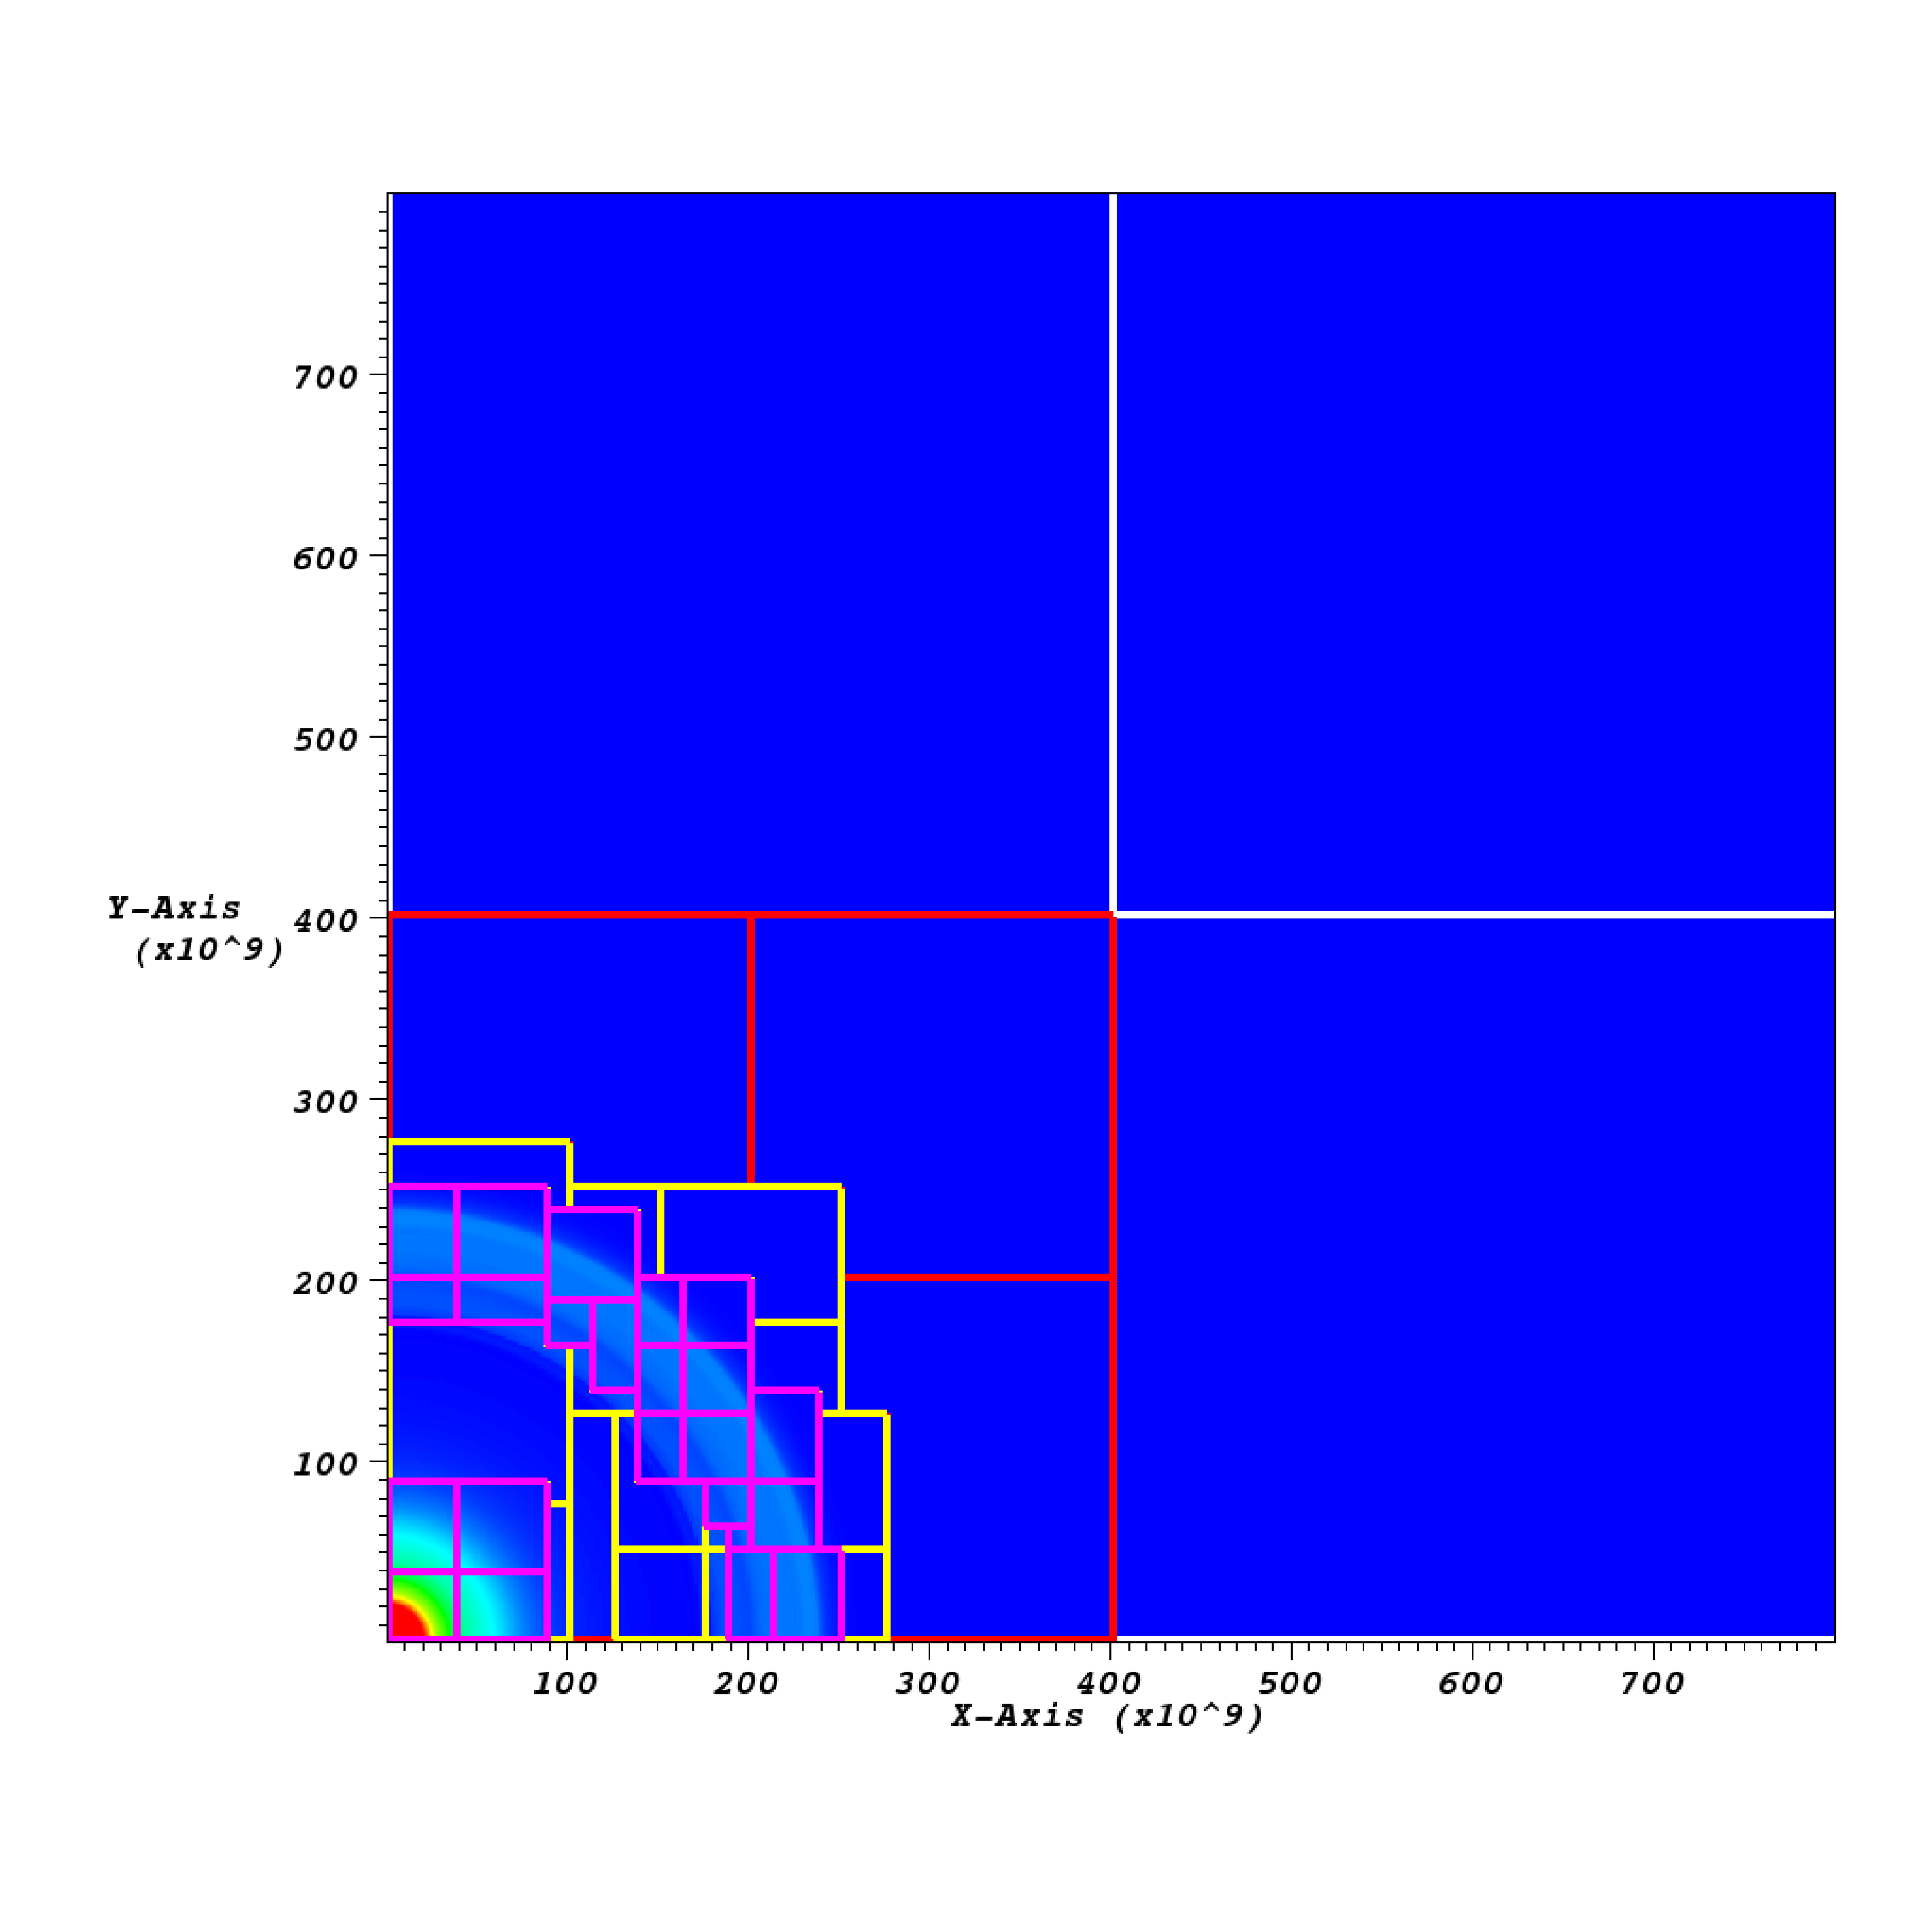
\includegraphics[width=3in]{ConvertCheckpoint/grown_corner_2}
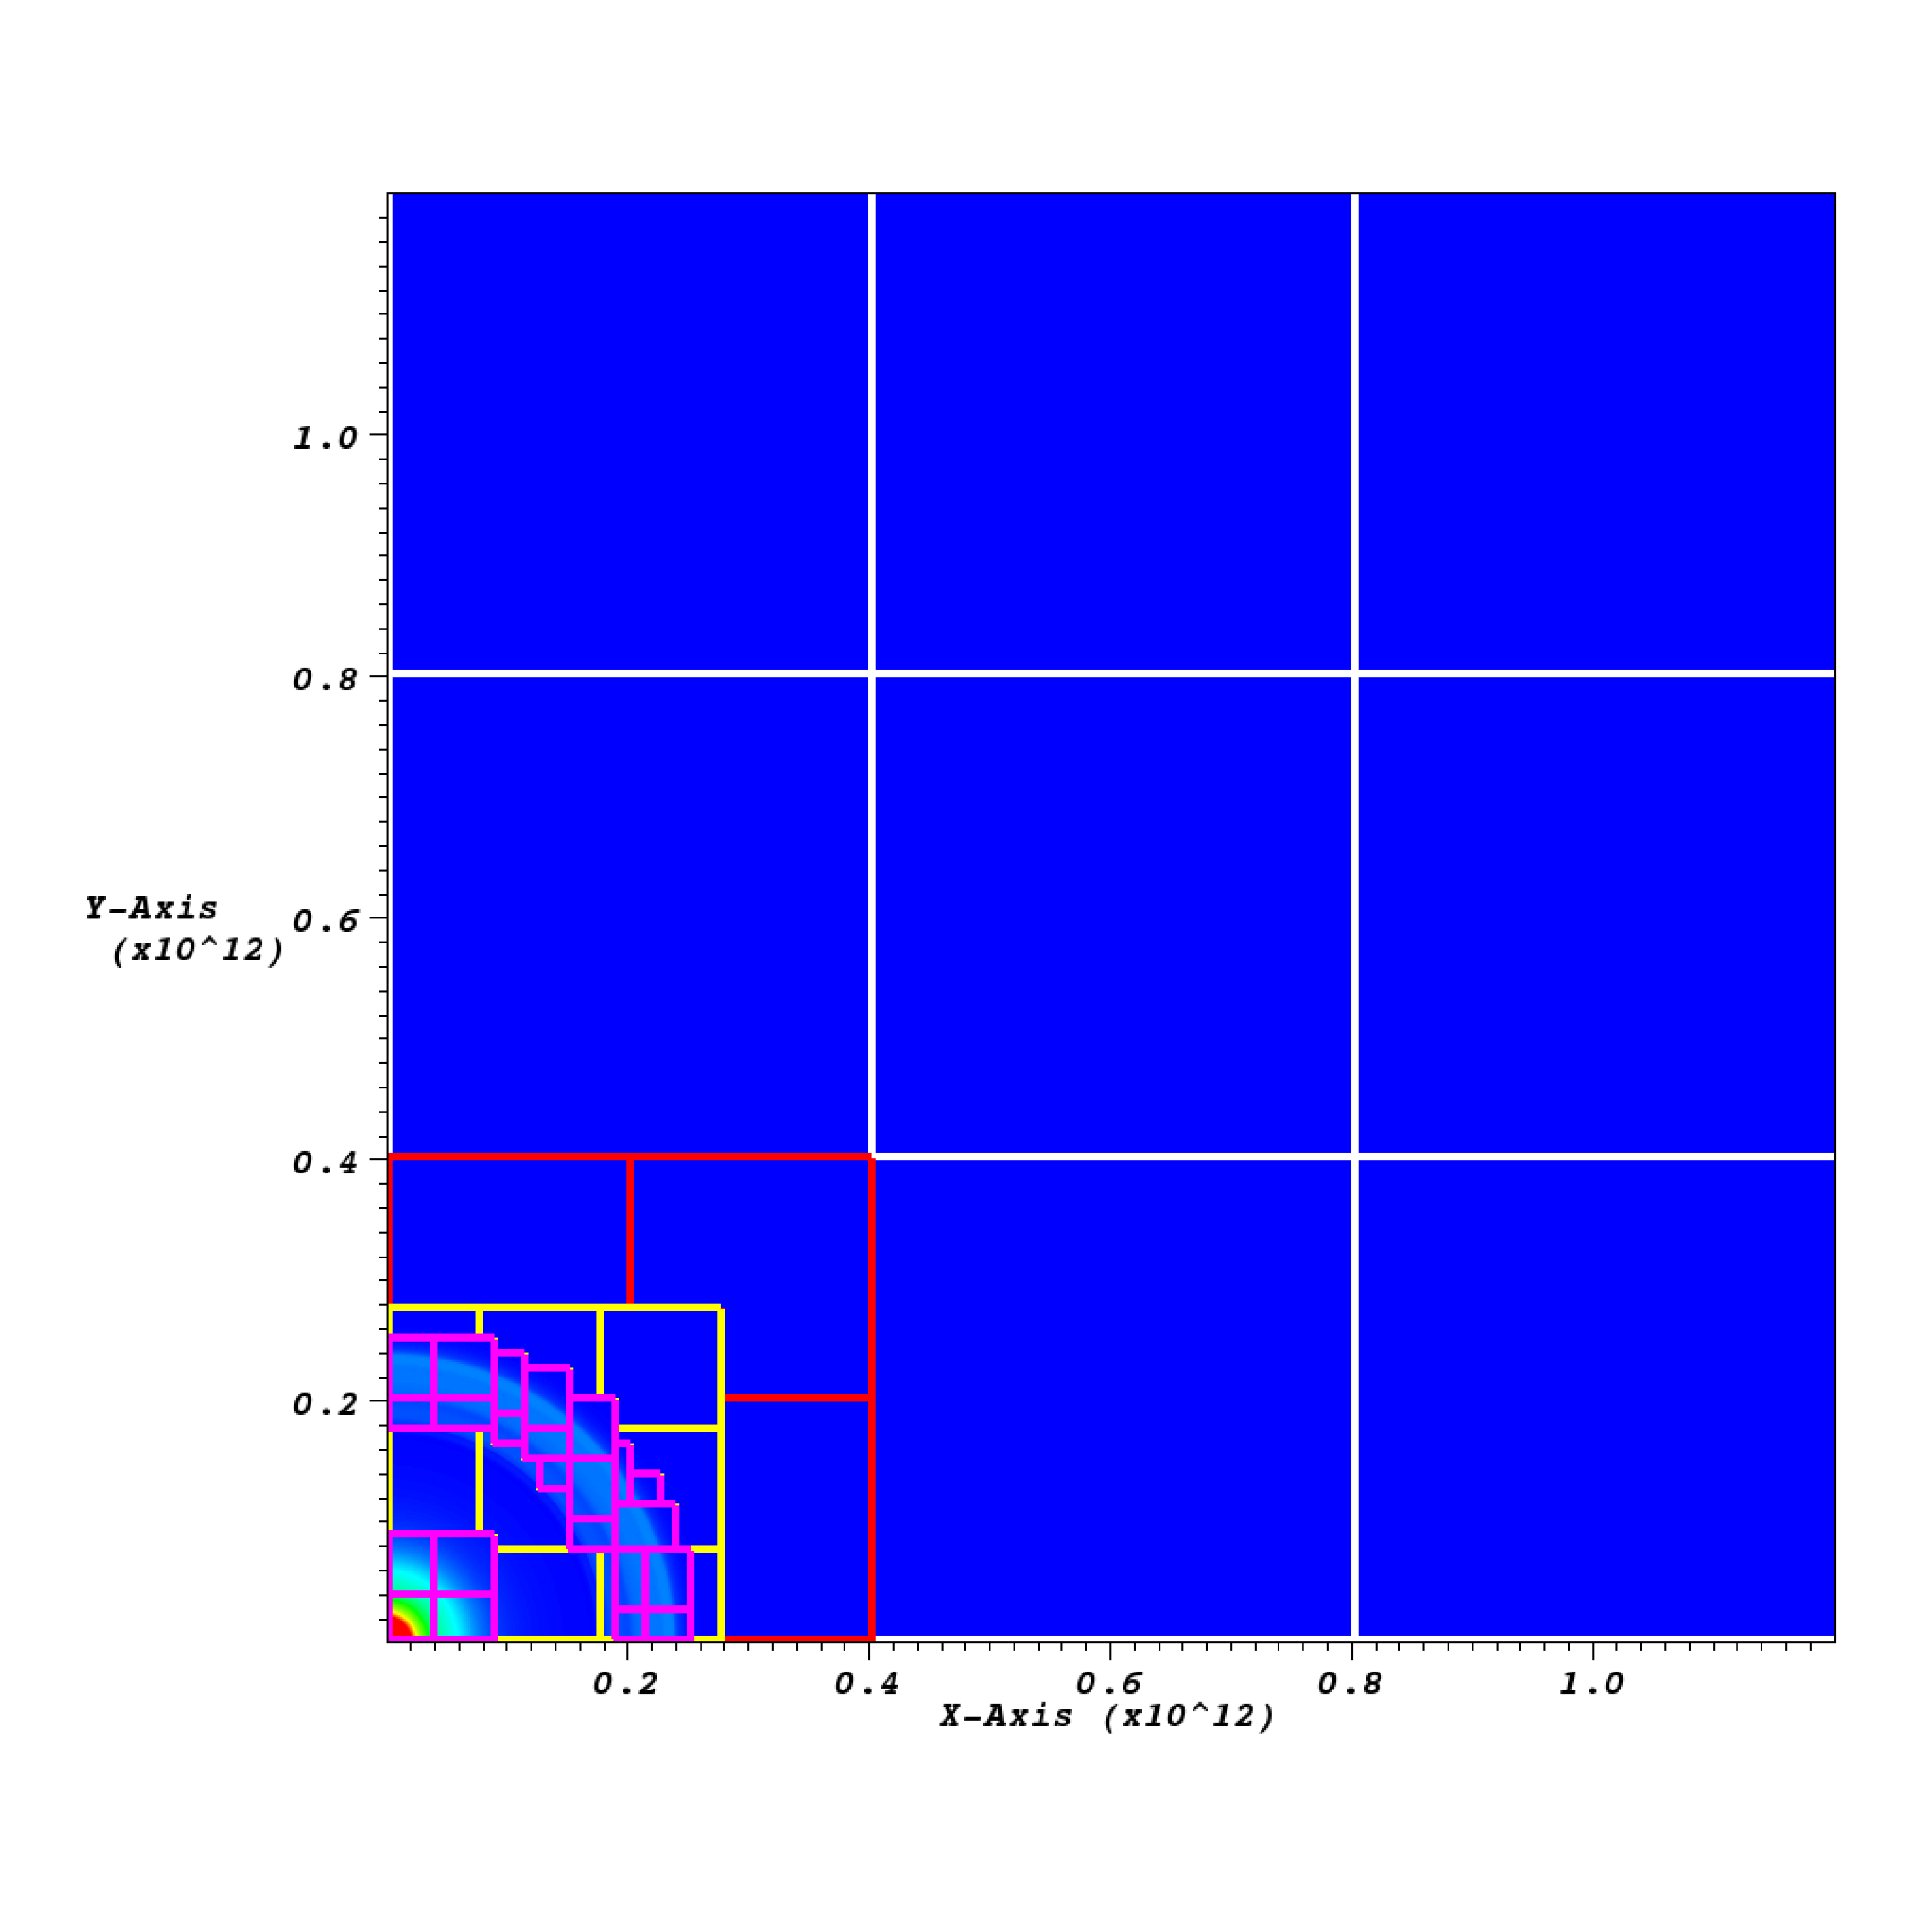
\includegraphics[width=3in]{ConvertCheckpoint/grown_corner_3}
\caption{Data from checkpoint file before and after the domain has been coarsened and grown.  This case
uses {\bf star\_at\_center = 0}  and {\bf ref\_ratio}=2.  The first grown example has 
{\bf grown\_factor}=2,  the second has {\bf grown\_factor}=3.  In all figures the level 0 grids 
are shown in white, the level 1 grids in red, the level 2 grids in yellow, and in the grown figures, 
the level 3 grids are in pink.}
\end{figure}
%%%%%%%%%%%%%%%%%%%%%%%%%%%%%%%%%

%%%%%%%%%%%%%%%%%%%%%%%%%%%%%%%%%
\begin{figure}[h]
\centering
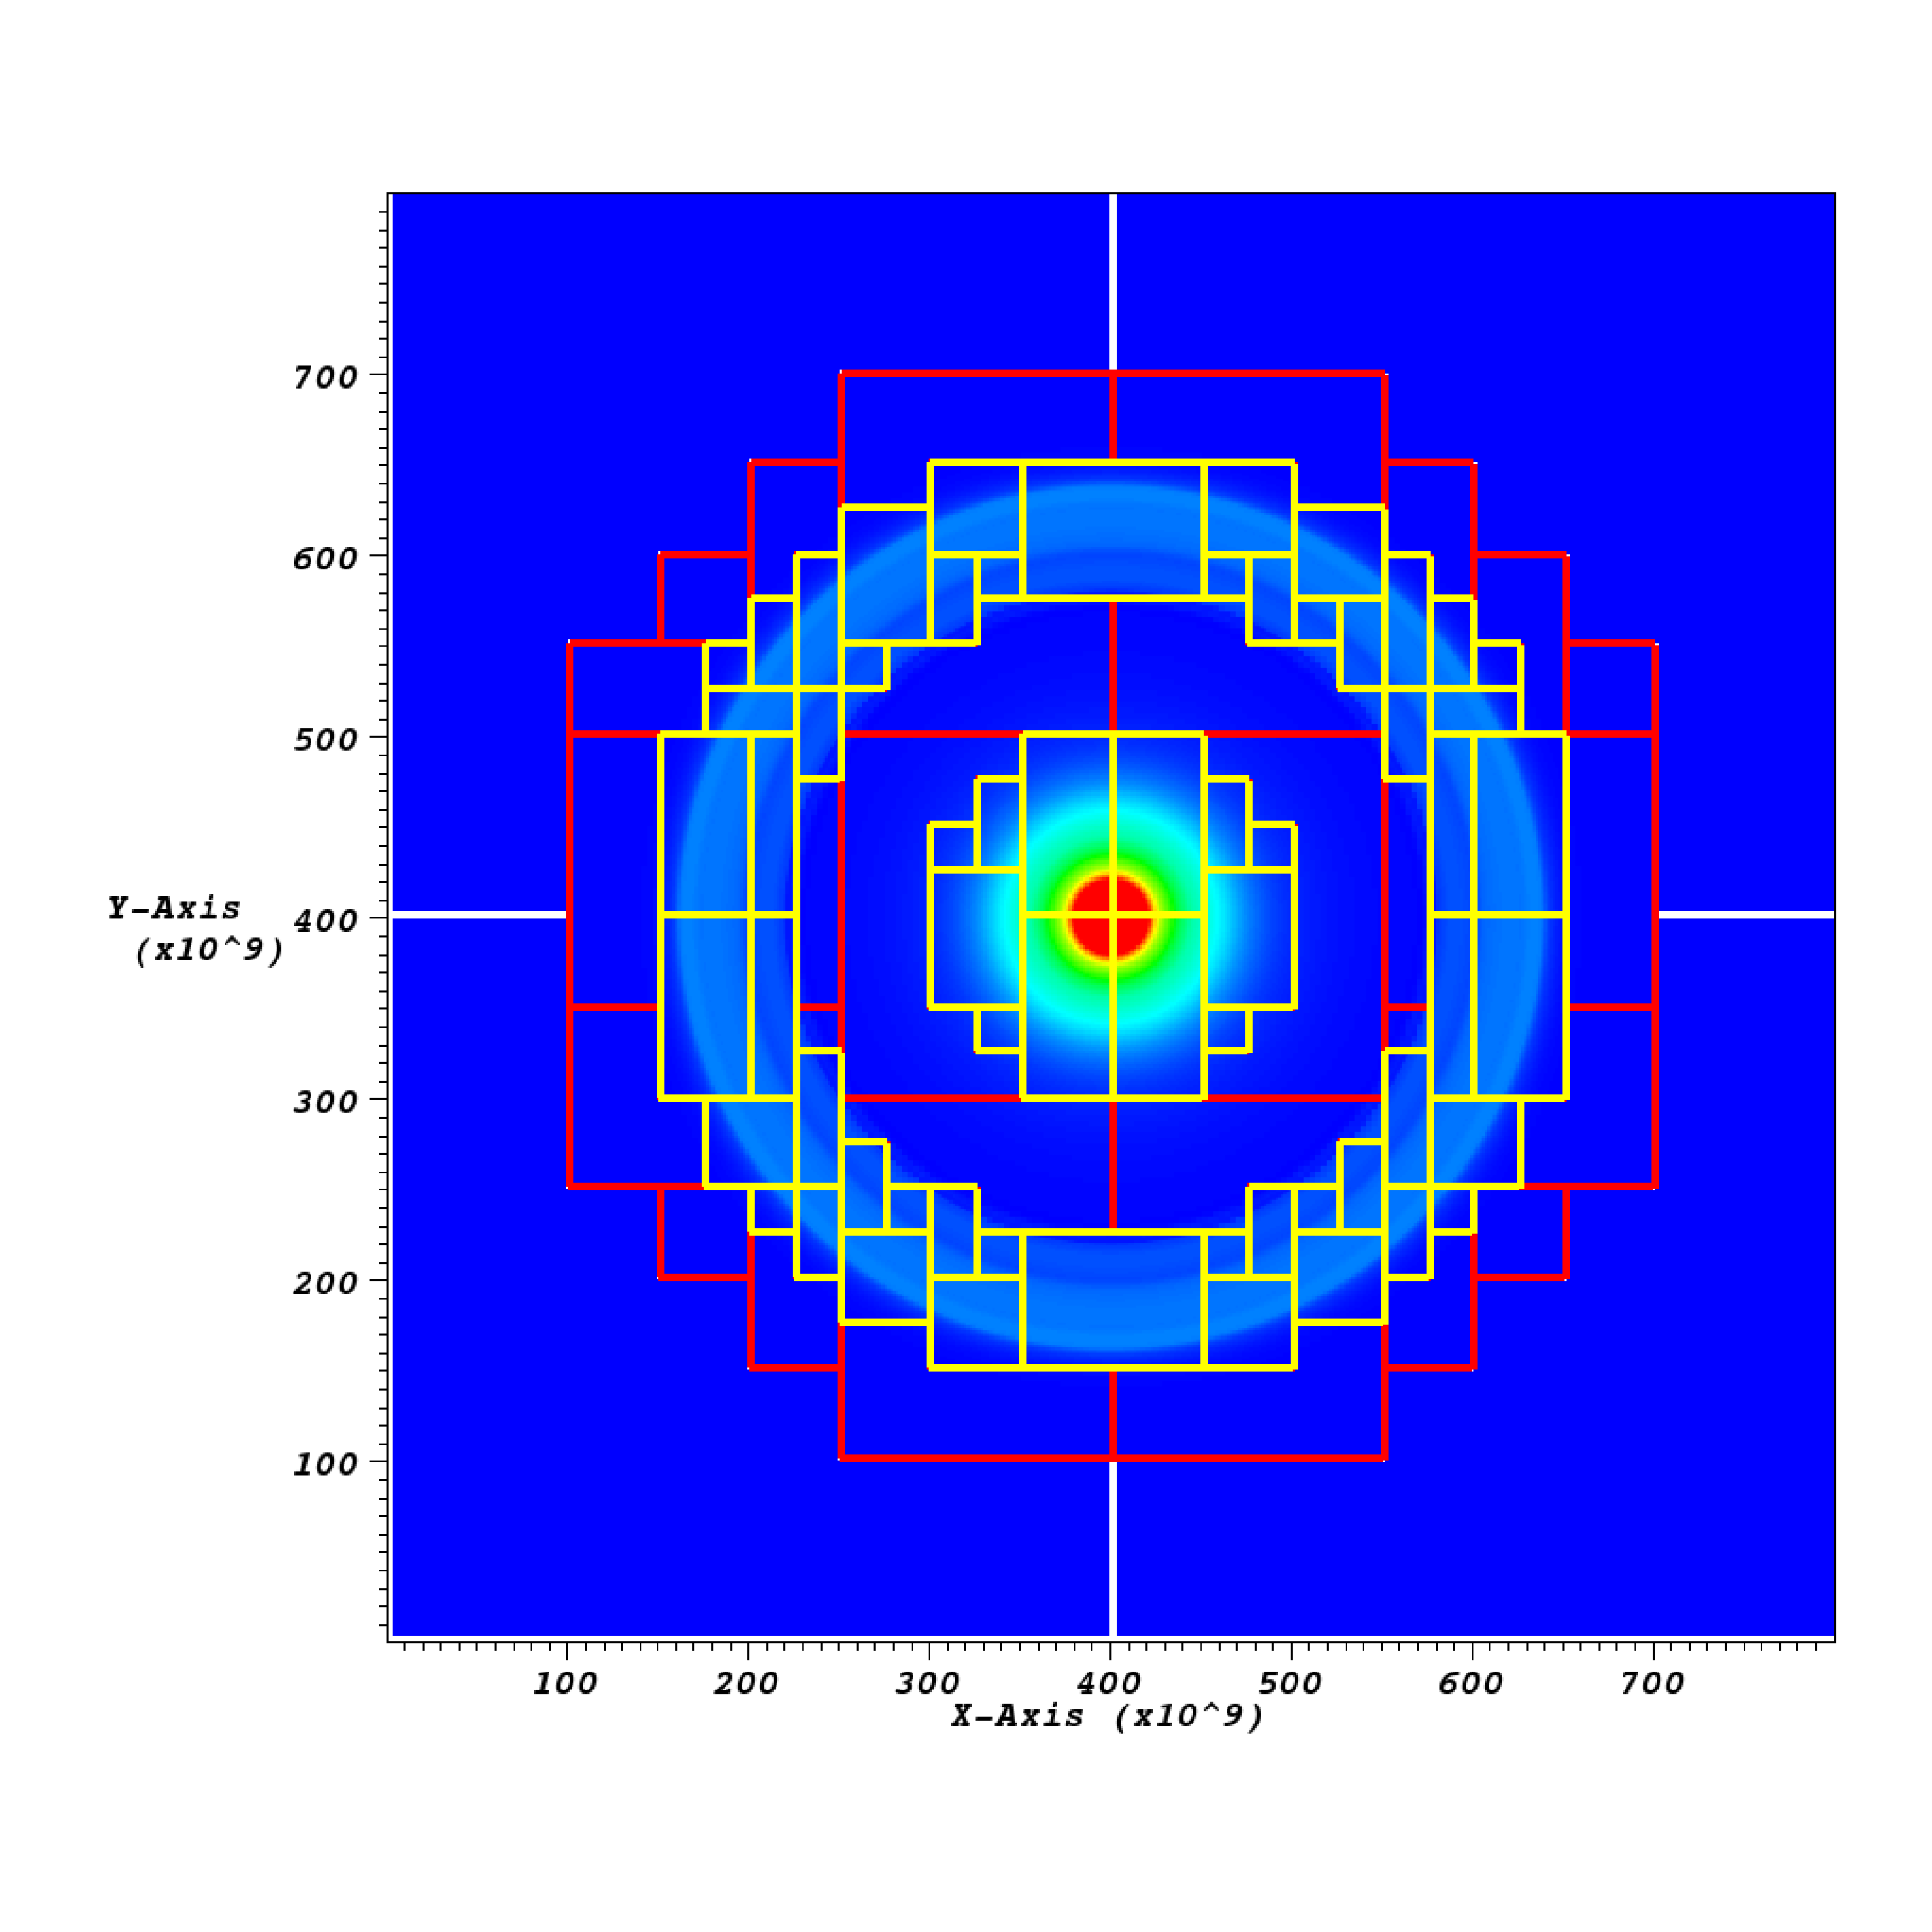
\includegraphics[width=3in]{ConvertCheckpoint/orig_center}
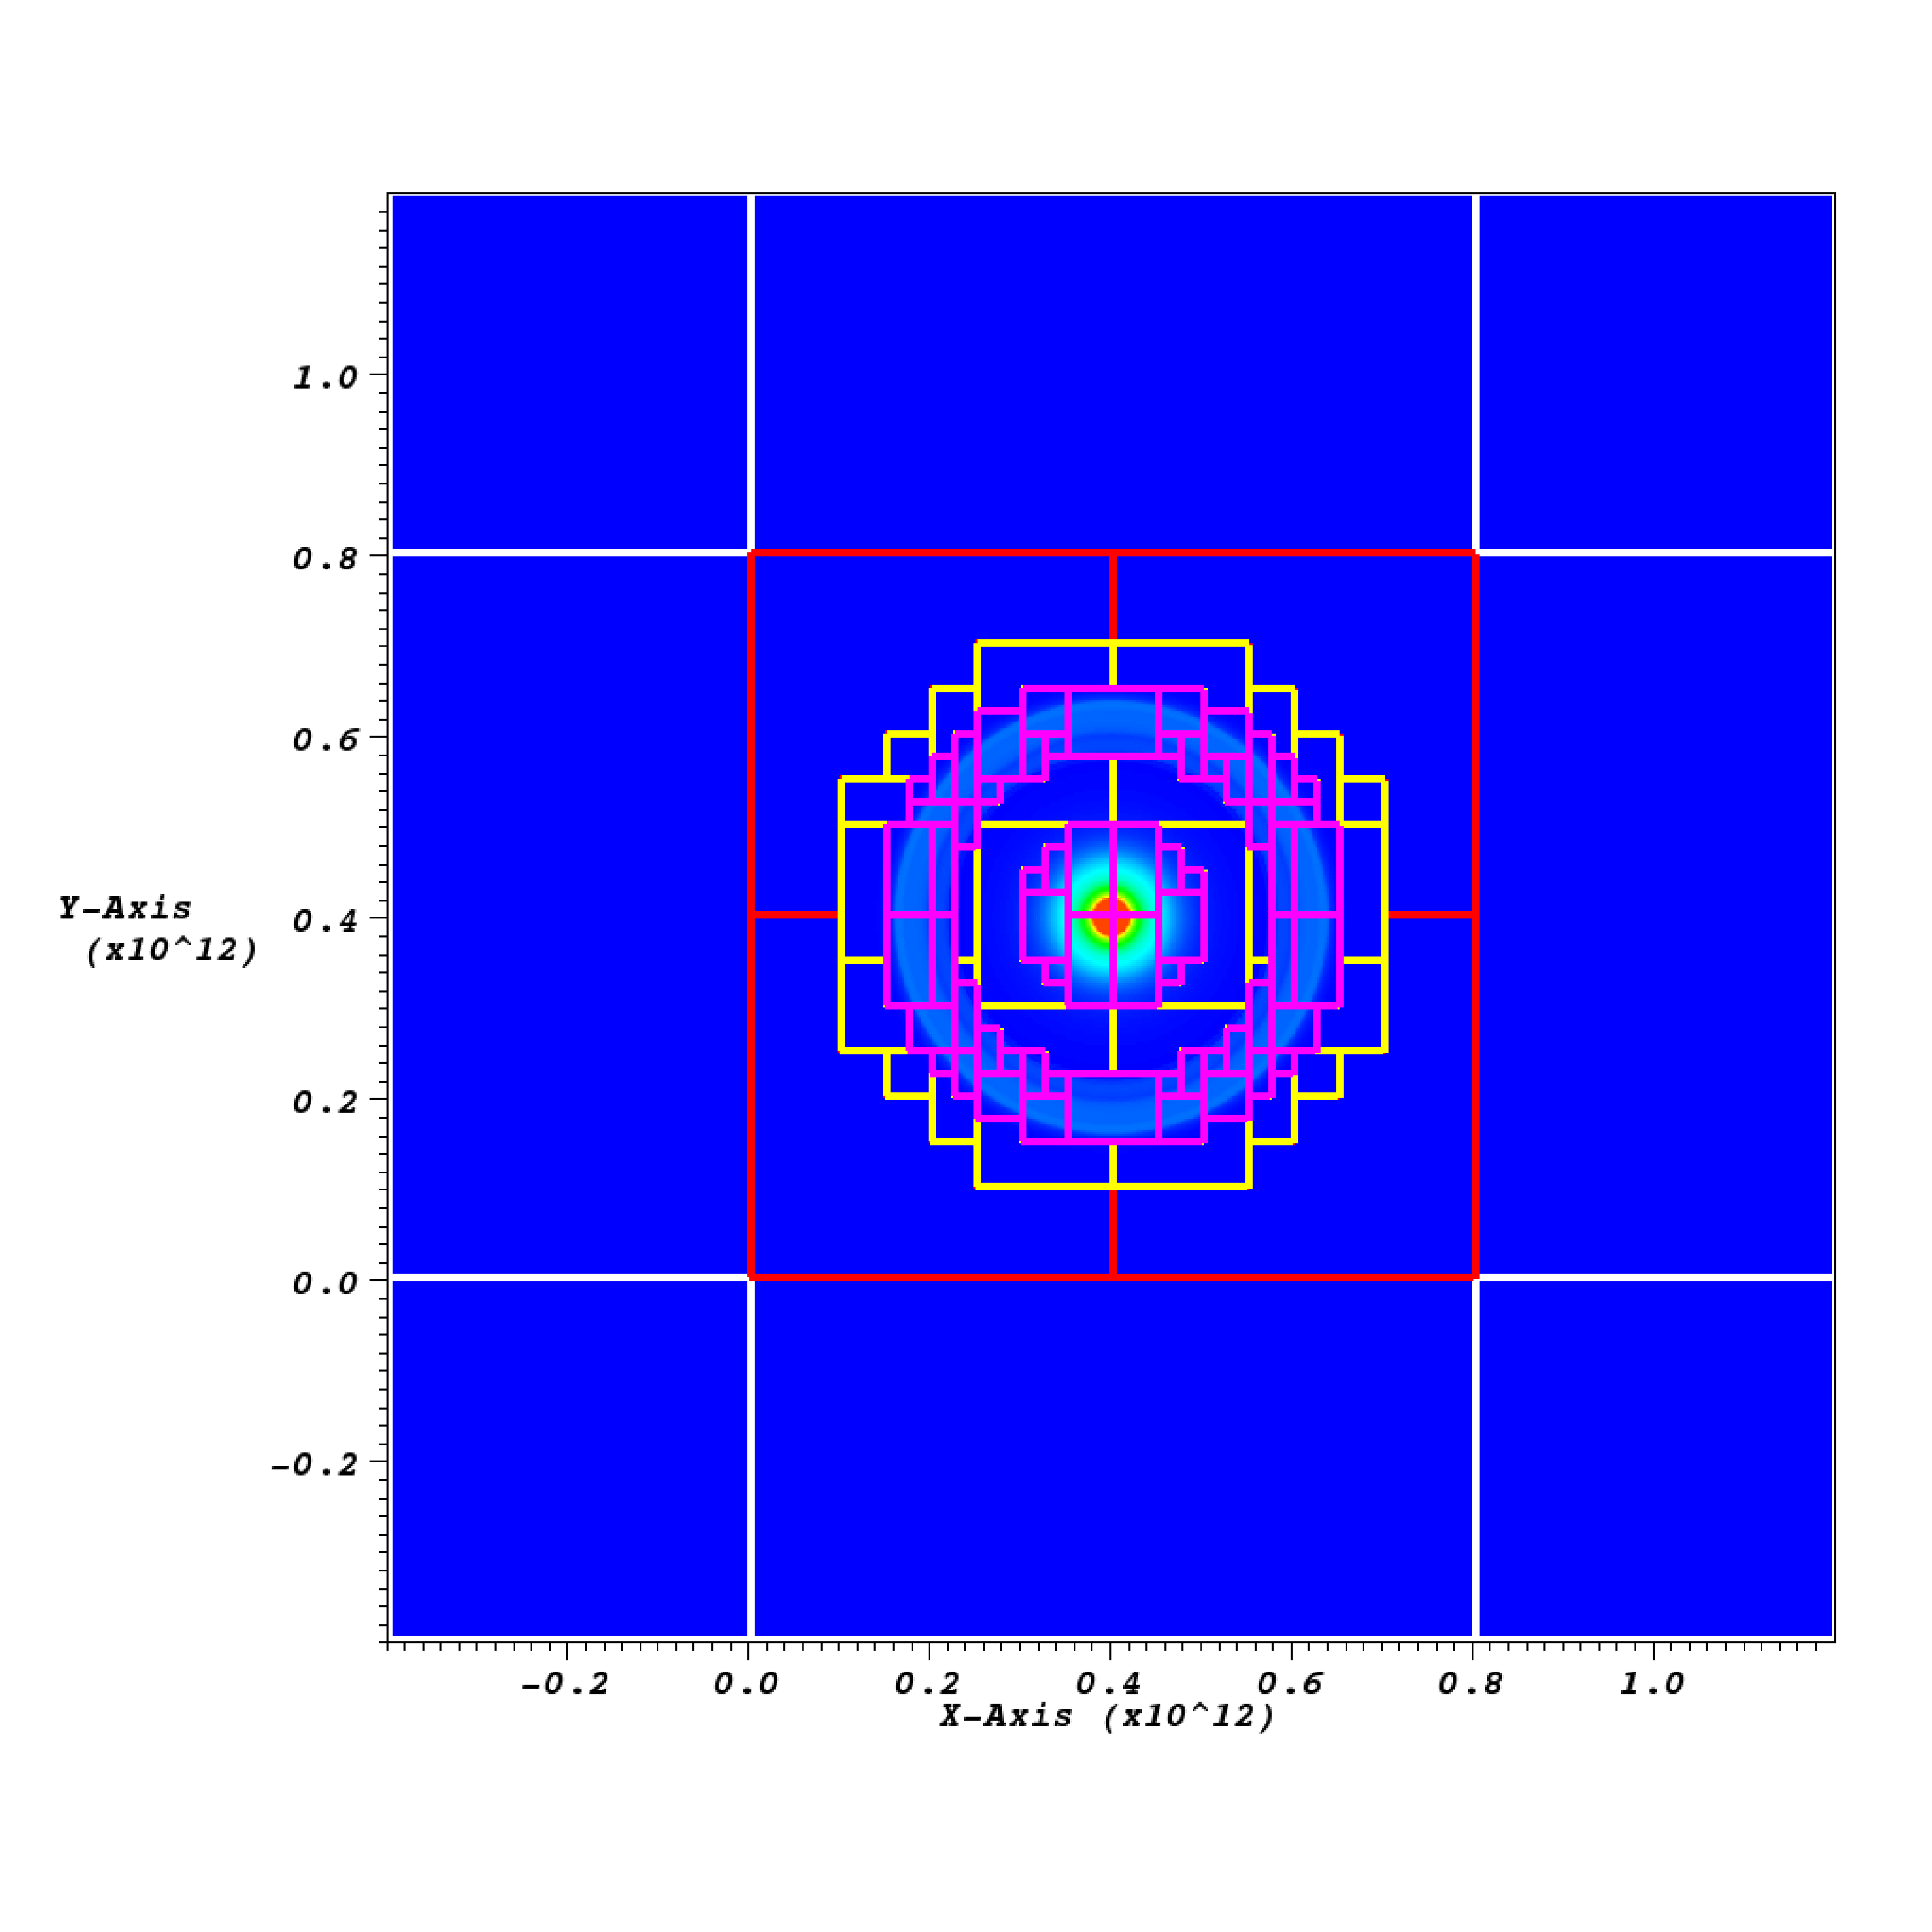
\includegraphics[width=3in]{ConvertCheckpoint/grown_center_2}
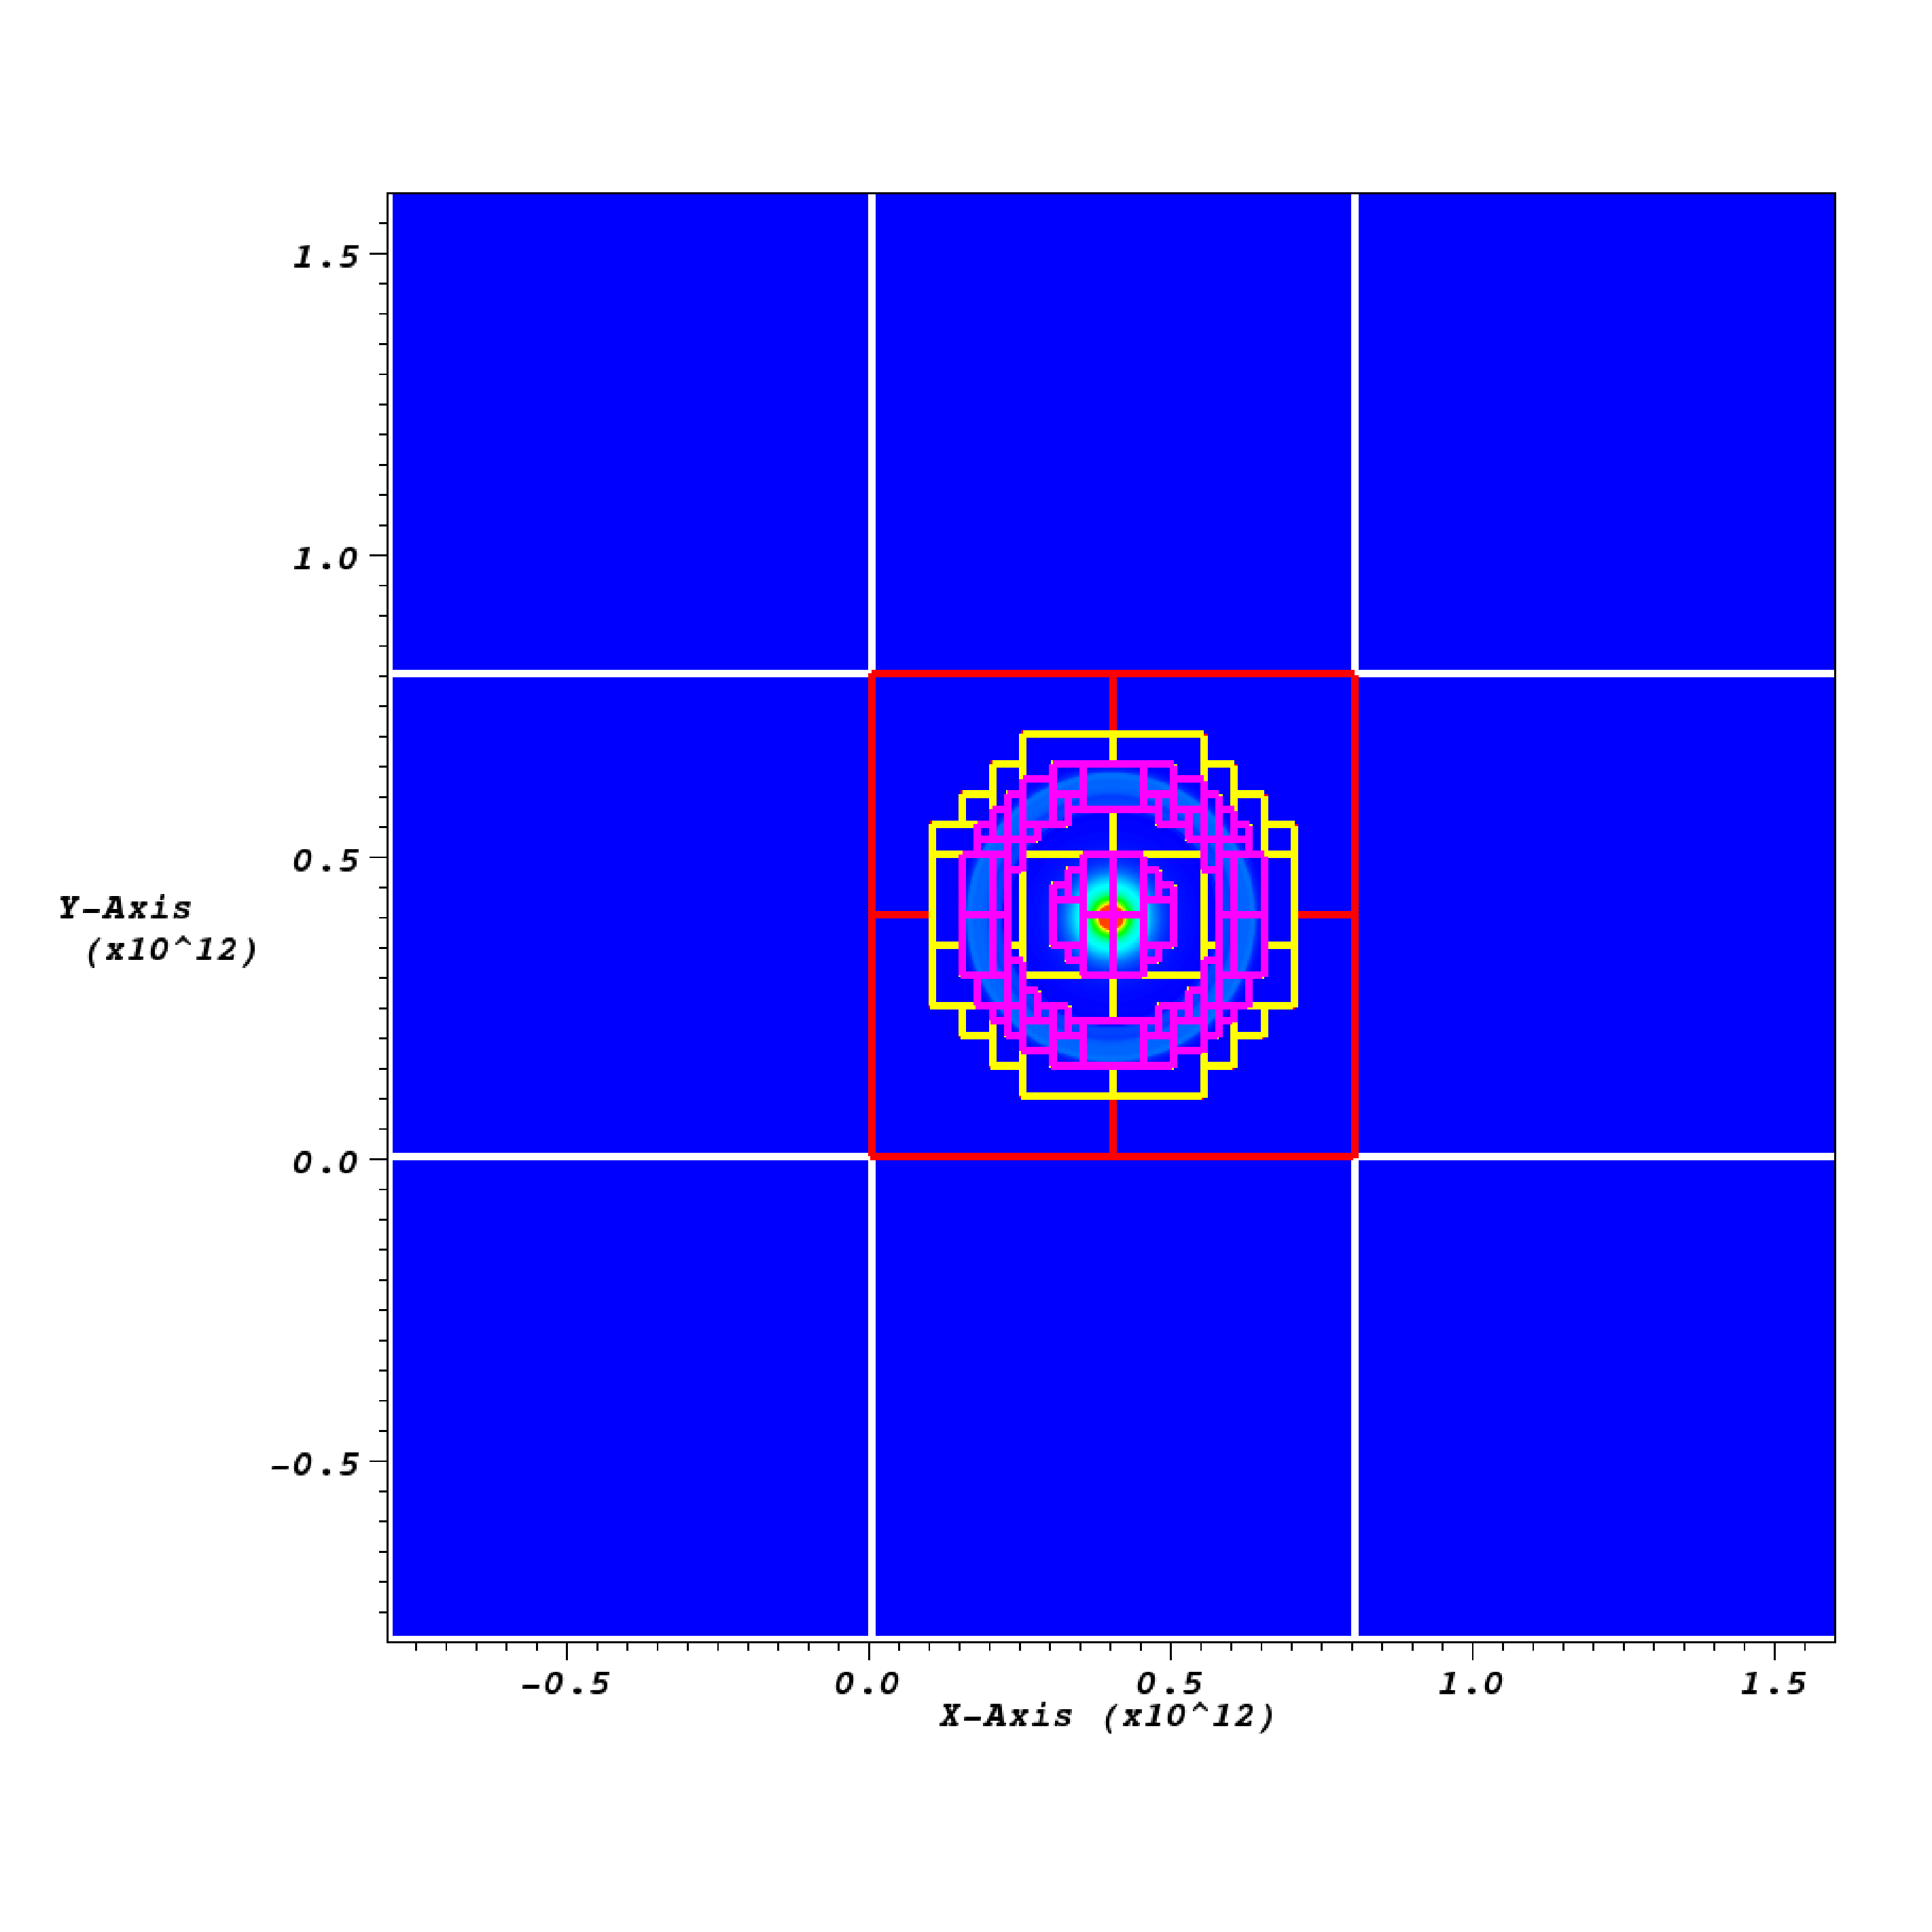
\includegraphics[width=3in]{ConvertCheckpoint/grown_center_3}
\caption{Data from checkpoint file before and after the domain has been coarsened and grown.  This case
uses {\bf star\_at\_center = 0}  and {\bf ref\_ratio}=2.  The first grown example has 
{\bf grown\_factor}=2,  the second has {\bf grown\_factor}=3.  In all figures the level 0 grids 
are shown in white, the level 1 grids in red, the level 2 grids in yellow, and in the grown figure, 
the level 3 grids are in pink. }
\end{figure}
%%%%%%%%%%%%%%%%%%%%%%%%%%%%%%%%%

